% \documentclass[aspectratio=169]{beamer}
\documentclass{beamer}

% \setbeameroption{show only notes}
\usepackage[utf8]{inputenc}
\usetheme{metropolis} 
\usepackage{graphicx}
\graphicspath{{../images}}
\usepackage{amsmath,amssymb,amsfonts}
\usepackage{multirow}
\usepackage{booktabs}  
\usepackage{adjustbox}
\usepackage{lmodern}
\usepackage[UTF8]{ctex}
% \usepackage[english]{babel}
\usepackage{pgfpages}

% 这里取消默认 note 页面的 header、footer 等
\setbeamertemplate{note page}{%
  % 用一个简单的 box 显示当前 slide 的 frametitle(如果没有 frametitle,这行可以省略)
  \ifx\insertframetitle\empty
  \else
    \vspace*{1em}%
    {\usebeamercolor[fg]{frametitle}\usebeamerfont{frametitle}\insertframetitle\par}%
    \vspace{1em}%
  \fi
  % 然后显示笔记内容
  Note:

  \insertnote%
}

\title{电影推荐系统}
\subtitle{大数据分析技术期中开题报告}
\author{杨淳瑜,王海天,陈可豪,王熙同}
\date{\today}

\begin{document}


\begin{frame}
    \titlepage
\end{frame}

\begin{frame}
    \frametitle{目录}
    \tableofcontents
\end{frame}

\section{加权评分方法}

\begin{frame}
    \frametitle{加权评分方法}
    为什么要定义一种加权的评分方法?
    \begin{itemize}
        \item 只考虑评分:小众电影评分人少但分高,不准确
        \item 只考虑评分人数:烂片评分人多但分低,不准确
        \item 需要一种加权的评分方法,既能反映评分质量,又能反映评分人数
    \end{itemize}
\end{frame}

\begin{frame}
    \frametitle{数据集基础统计}
    \begin{table}
        \centering
        \begin{tabular}{ll}
            \toprule
            统计项     & 值           \\
            \midrule
            电影总数    & 45,463      \\
            年份范围    & 1874 - 2020 \\
            最高产年份   & 2014.0      \\
            平均评分    & 5.62 / 10   \\
            评分中位数   & 6.00 / 10   \\
            评分范围    & 0.0 - 10.0  \\
            平均投票次数  & 109.9       \\
            投票次数中位数 & 10.0        \\
            最高投票次数  & 14,075.0    \\
            平均时长    & 94.1 分钟     \\
            时长范围    & 0 - 1256 分钟 \\
            \bottomrule
        \end{tabular}
    \end{table}
\end{frame}

% \begin{frame}
%     \frametitle{评分分布}
%     \begin{table}
%         \centering
%         \begin{tabular}{lll}
%             \toprule
%             评分  & 数量     & 占比     \\
%             \midrule
%             0.5 & 1,101  & 1.1\%  \\
%             1.0 & 3,326  & 3.3\%  \\
%             1.5 & 1,687  & 1.7\%  \\
%             2.0 & 7,271  & 7.3\%  \\
%             2.5 & 4,449  & 4.4\%  \\
%             3.0 & 20,064 & 20.1\% \\
%             3.5 & 10,538 & 10.5\% \\
%             4.0 & 28,750 & 28.7\% \\
%             4.5 & 7,723  & 7.7\%  \\
%             5.0 & 15,095 & 15.1\% \\
%             \bottomrule
%         \end{tabular}
%     \end{table}
% \end{frame}

\begin{frame}
    \frametitle{基础评分公式}
    \[ WR = \left(\frac{v}{v+m}\right) \cdot R + \left(\frac{m}{v+m}\right) \cdot C \]

    \vspace{0.5cm}
    \textbf{参数说明}:
    \begin{itemize}
        \item $C$:全平台电影平均分(基准线)
        \item $m$:最小有效投票阈值,例如下95\%的位置
        \item $v$:当前电影实际投票数
        \item $R$:当前电影原始平均分
    \end{itemize}
\end{frame}

\begin{frame}
    \frametitle{参数分析}

    \begin{figure}
        \centering
        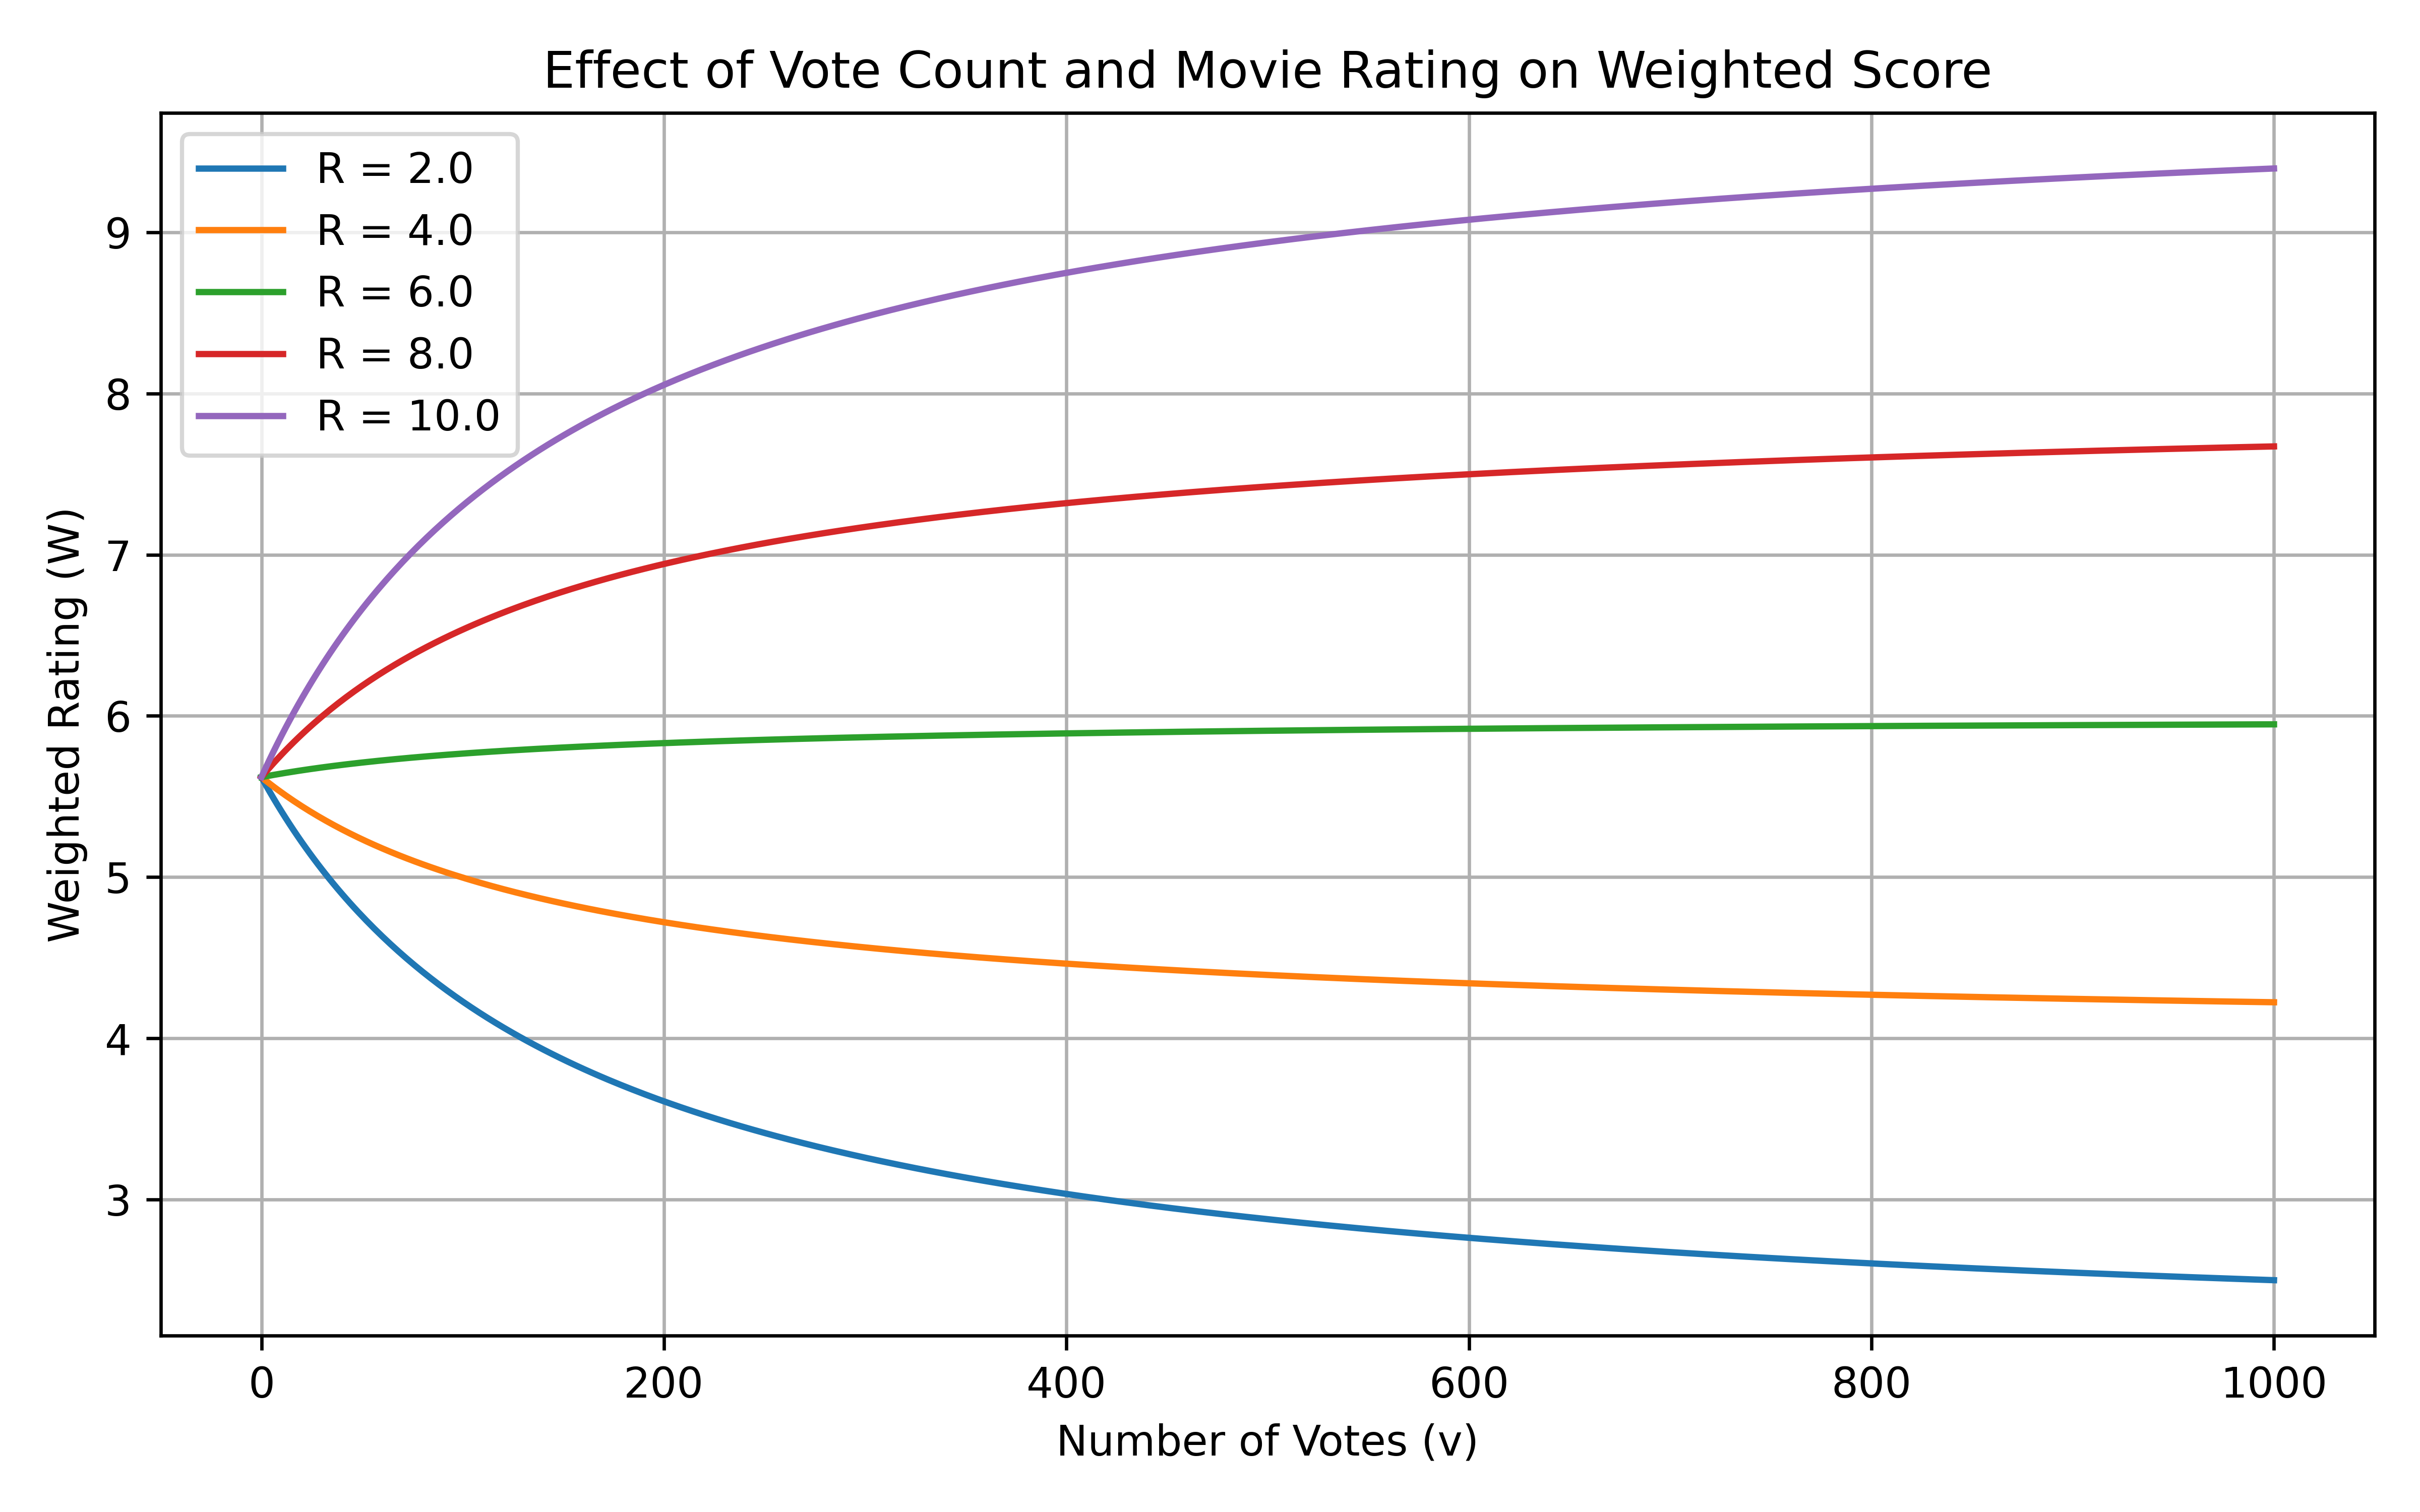
\includegraphics[width=0.7\textwidth]{weighted_rating.png}
        \caption{参数分析}
    \end{figure}

    由于均值是评分5.62:
    \begin{itemize}
        \item 当$R$小于5.62的时候,评分人数越多,$WR$越小
        \item 当$R$大于5.62的时候,评分人数越多,$WR$越大
    \end{itemize}

\end{frame}

\section{相似性推荐}

\begin{frame}
    \frametitle{相似性推荐}
    核心思路:对剧情文本进行清洗,然后向量化,然后计算余弦相似度。

    \vspace{0.5cm}
    向量化的方法由简单到复杂,我们计划使用:
    \begin{itemize}
        \item TF-IDF
        \item BERT
    \end{itemize}
\end{frame}

\begin{frame}
    \frametitle{向量化:TF-IDF}
    \textbf{核心步骤}:
    \begin{enumerate}
        \item 使用TF-IDF算法进行向量化
        \item 计算剧情向量间的余弦相似度
        \item 基于相似度排序,生成Top-K推荐
    \end{enumerate}

    \textbf{核心算法}:
    \begin{itemize}
        \item TF-IDF权重计算:
              \[ w_{ij} = \mathrm{TF}(t_j,d_i) \times \log\frac{N}{\mathrm{DF}(t_j)} \]
        \item 余弦相似度:与文本长度无关, Scaling Invariant
              \[ \cos(\theta) = \frac{\vec{A} \cdot \vec{B}}{\|\vec{A}\| \|\vec{B}\|} \]
    \end{itemize}
\end{frame}

\begin{frame}
    \frametitle{向量化:BERT}
    \textbf{技术路线}:
    \begin{enumerate}
        \item 采用Huggingface上的轻量级RoBERTa预训练模型
        \item 对电影剧情文本进行语义向量编码
        \item 使用余弦相似度计算电影语义相似性
        \item 生成基于深度语义的推荐结果
    \end{enumerate}
\end{frame}

\section{关联规则推荐}

\begin{frame}
    \frametitle{FP-Growth算法流程}
    \textbf{实现步骤}:
    \begin{enumerate}
        \item 转换用户评分行为数据为事务数据集
        \item 构建FP-Tree压缩数据结构
        \item 递归挖掘频繁项集
        \item 生成高质量关联规则
        \item 根据置信度和加权评分的综合分数进行筛选和排序
    \end{enumerate}
\end{frame}

\begin{frame}
    \frametitle{有效规则定义}

    \vspace{0.5cm}
    \textbf{应用策略}:
    \begin{itemize}
        \item 最小支持度:0.06
        \item 最小置信度:0.3
        \item 规则排序:置信度优先
    \end{itemize}

    FP-Tree离线生成,用户输入电影名称,我们查询挖掘到的规则中,以该电影为前件的规则,然后根据置信度排序,生成Top-K推荐。

    更进一步,我们可以允许前件有多个电影,用户的输入也可以是多个。
\end{frame}




% \section{混合推荐策略}

% \begin{frame}
% \frametitle{混合推荐策略}
% \textbf{综合评分公式}:
% \[ Score_{final} = \alpha \cdot WR + (1-\alpha) \cdot Similarity \]

% 或者是

% \[ Score_{final} = \alpha \cdot WR + (1-\alpha) \cdot Confidence \]

% 其中:
% \begin{itemize}
%     \item $WR$为加权评分方法得分
%     \item $Similarity$为相应推荐方法的相似度分数
%     \item $\alpha$为平衡参数,控制评分与相似度(置信度)的权重
% \end{itemize}
% \end{frame}

% \begin{frame}
% \frametitle{谢谢}
% \begin{center}
%     \Huge{谢谢}
% \end{center}
% \end{frame}


\end{document}

